\title{G53FIV Report}
\author{
  Jack Ellis \\
  psyje5@nottingham.ac.uk\\
  4262333
}
\date{}
\documentclass[12pt]{article}
\usepackage{graphicx}
\graphicspath{ {../Images/} }
\usepackage{mathtools}
\usepackage[rightcaption]{sidecap}

\newcommand{\myfig}{\begin{SCfigure}[0.7][p]}


  \begin{document}
  \maketitle
  \tableofcontents
  \pagebreak

  \section{Description of Data}
  The dataset I shall be using is the \verb|tsort.info/music| collection of data of the world music charts. 
  This is a \textasciitilde 71000 line CSV file containing information about albums and songs, recording the top 100 songs and albums from most years, as well as anything by the top 1000 artists (including collaborations). 
  \\
  Per the website, this information is collated from 227 different data sources, 135 song charts and 92 album charts from Australia, Austria, Belgium, Brazil, Canada, Denmark, Eire, Finland, France, Germany, Holland, Italy, Japan, New Zealand, Norway, Poland, South Africa, Spain, Sweden, Switzerland, the UK and the US as well as some global and internet based listings to give the songs and albums that have topped the charts around the world for the last 116 years. The source data includes all the hits of 35,703 song artists and 21,867 album artists. 
  The columns are as follows:
  \begin{itemize}
    \item artist: The name of the artist
    \item name: The name of the entry (song or album title)
    \item type: The type of the entry, either song or album
    \item year: The year allocated to the entry (may be unknown)
    \item score: The score that this item achieved (this number may be preceeded by a space, this allows a text sort to get the values in the appropriate order)
    \item songentry\_pos: The song's position in the Top Songs list (or the empty string if it is not in it)
    \item songyear\_pos: The song's position in its Song Year list
    \item songartist\_pos: The artist's position in the Top Artists list (note that only the artist's top song is labeled in this way)
    \item songtitle\_pos: The song title's position in the Top Titles list (note that only the most highly placed cover version is labeled for each title)
    \item songdecade\_pos: The song's position in its Song Decade list
    \item namsong\_pos: The song's position in the Top North American Songs list for its year
    \item eursong\_pos: The song's position in the Top European Songs list for its year
    \item albumentry\_pos: The album's position in the Top Albums list
    \item albumyear\_pos: The album's position in its Album Year list
    \item albumartist\_pos: The artist's position in the Top Album Artists list (note that only the artist's top album is labeled in this way)
    \item albumdecade\_pos: The album's position in its Album Decade list
    \item notes: The chart entries for this item
  \end{itemize}

  \section{Initial Questions \& Visualisation Strategies}
  \subsection{Has music been getting better over the years?}
        This question requires that the ratings for each song be known, or at the very least a reasonable average of song quality according to reviewers be able to be made available.
        Bearing in mind the importance of not only seeing the average scores but also the lower and upper bounds of ratings over the time, a box plot is the most suitable visualisation.
        For this visualisation, we must decide on an interval from which to draw our visualisation.
        Per year would result in 50 boxes, not ideal for the visualisation on readibility grounds.
        Per decade would only give 5 points on x, which could lead to difficulty establishing a trend.
        Per 5 years is a good middle ground between these.
        To get the data to a usable point, all columns other than year and score were dropped, and years were rounded to the nearest 5.
        Albums were taken out of consideration as well, as they can often be rated differently to songs and this is another independent variable which we do not want.
        Using geom\_boxplot() we can visualise the median, quartile, and extreme values, as well as outliers of the data.\\
        \myfig
          \caption{Box Plot to show distribution of scores against half-decade of release}
          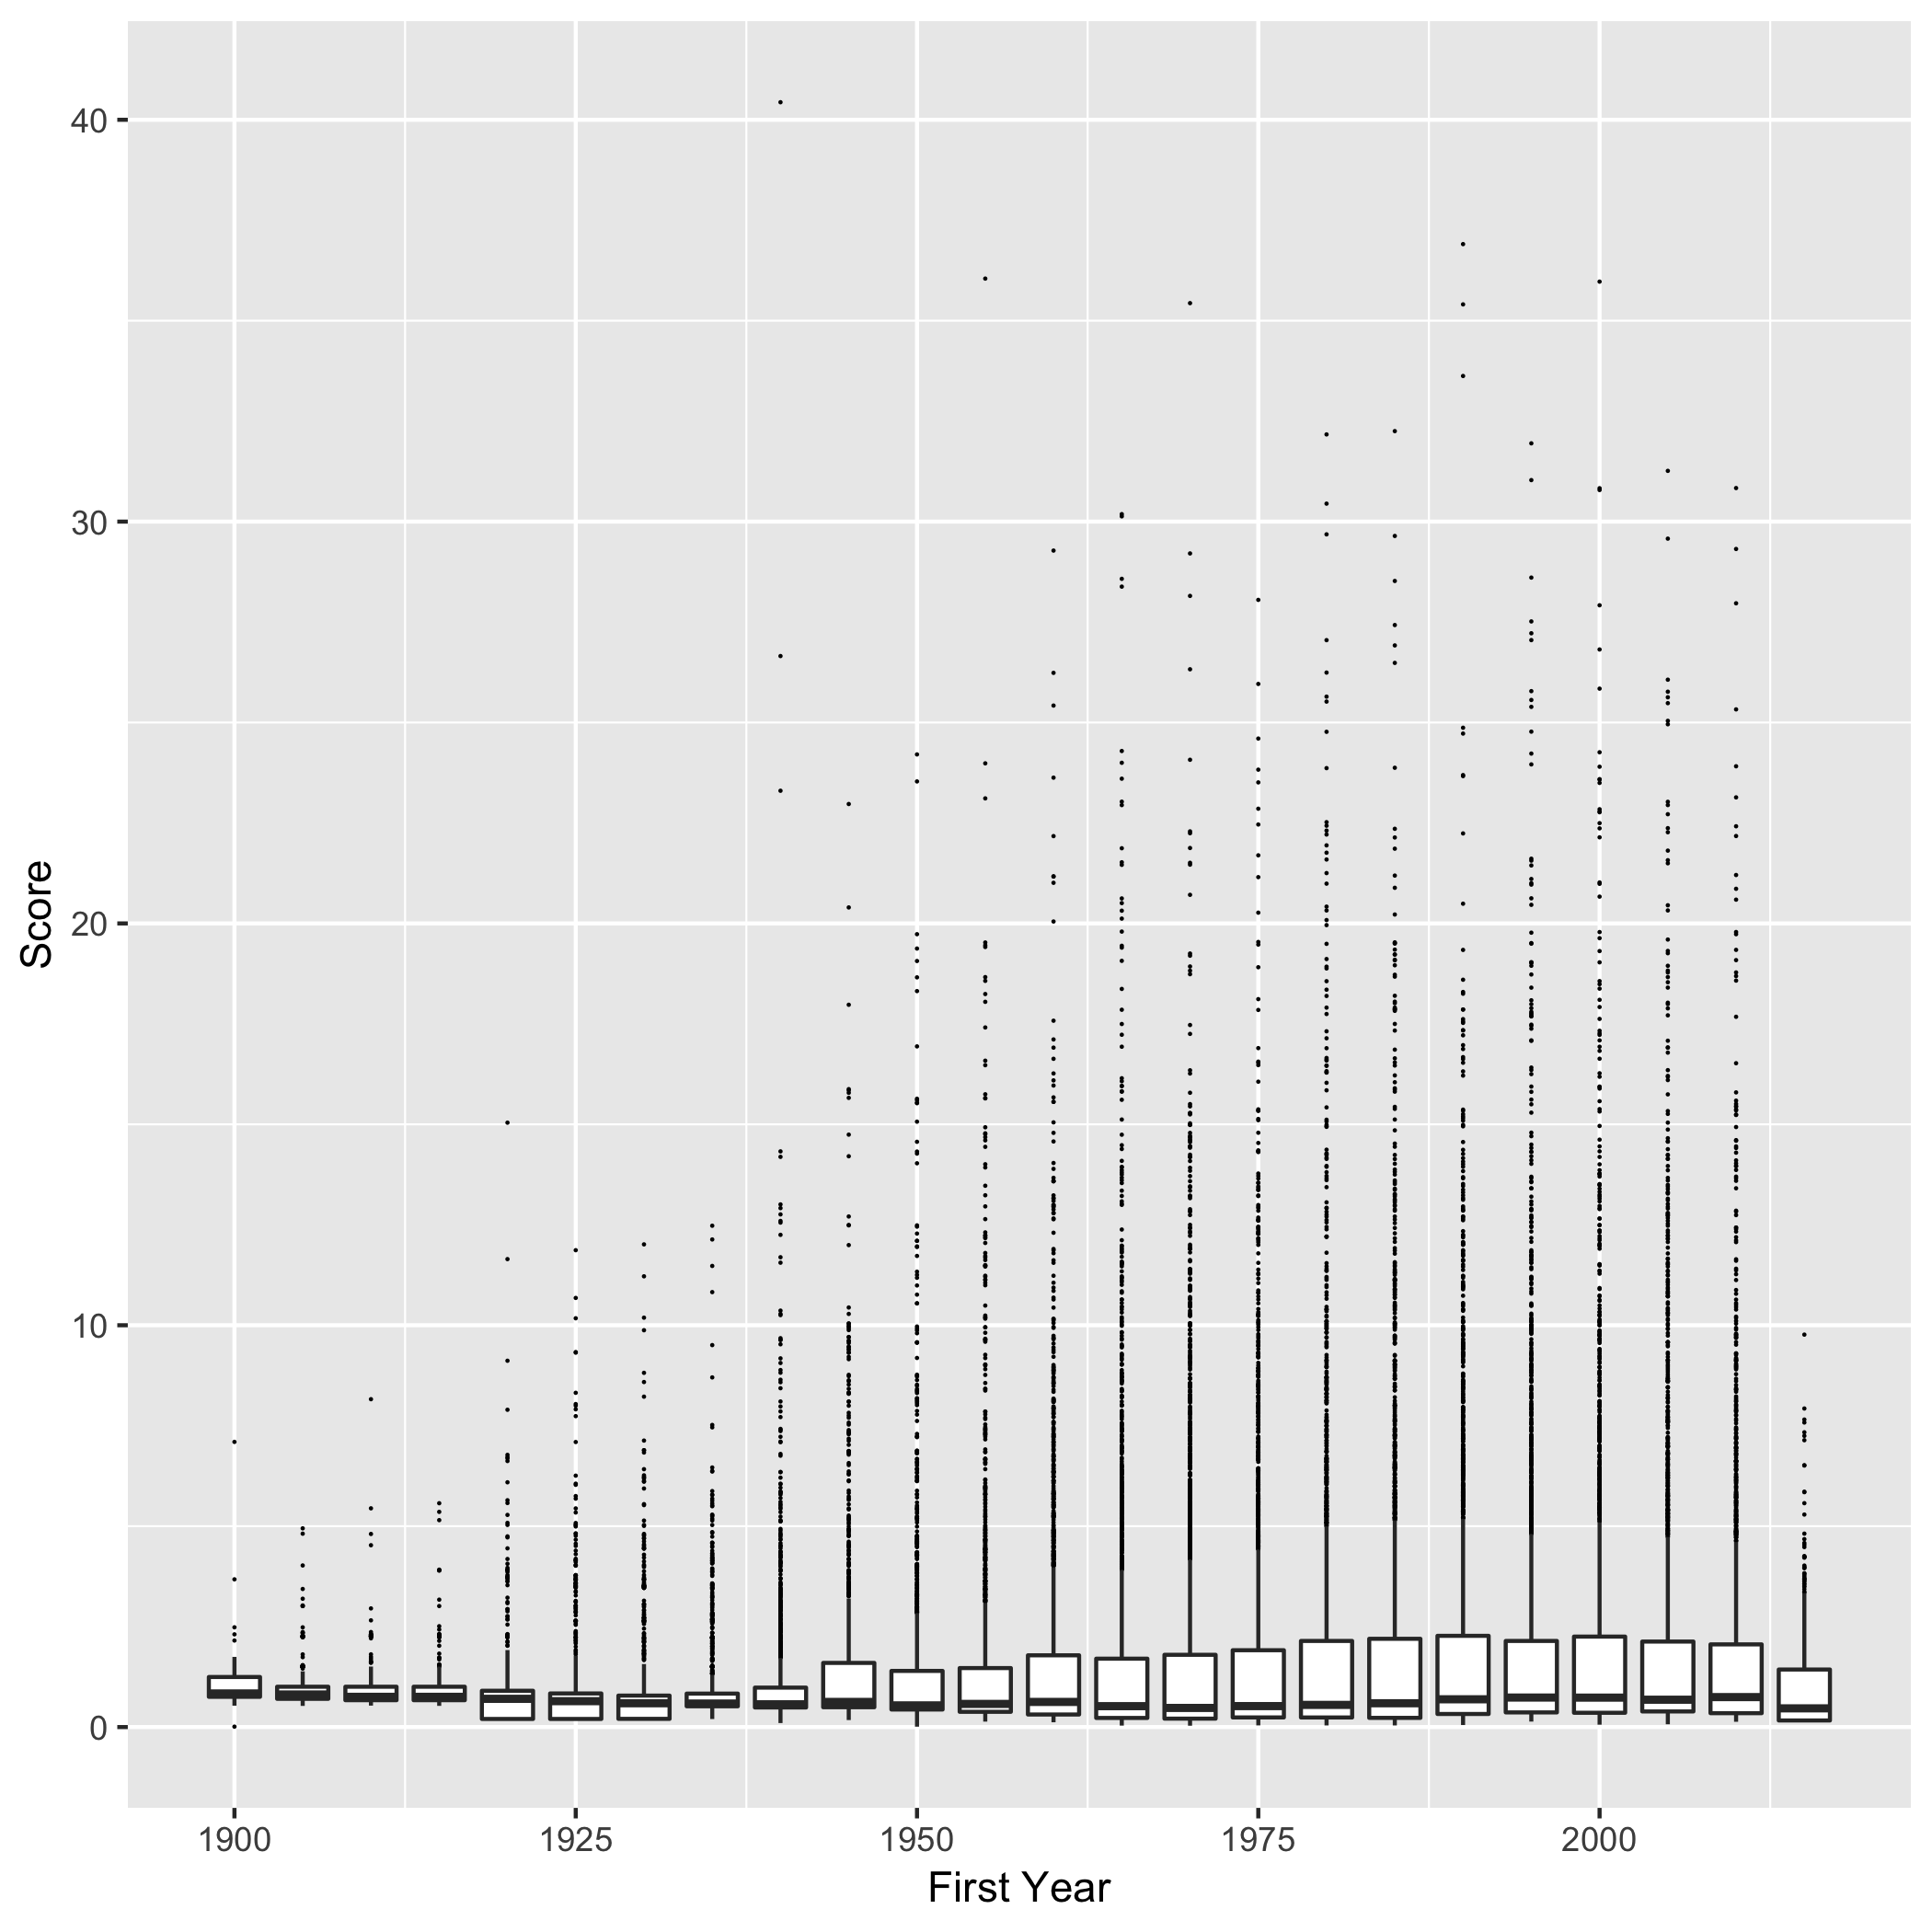
\includegraphics[width=0.5\textwidth]{yearScore}
          \label{fig:q1}
  \end{SCfigure}
        As we can see in Figure \ref{fig:q1}, the median values do not follow any appreciable trend, however as the half-decades go on there appear to be an increasing number of upward outliers, as well as a large increase in interquartile range.
        From this, we can establish that the quality of music has become more varied through the years, however the median quality has remained relatively steady.


  \subsection{Does a song's score from reviewers have any bearing on how well it sells?}
        This is a considerably easier question to answer; score and position on the Top 100 of the year/decade are all continuous variable, and consequently we can plot this information as a scatter graph.
        The only data manipulation that needs to be done here is to drop all rows that do not have a \verb|songyear_pos| value attached to them.

        \myfig
          \caption{Scatter graph to show position in Year-Top-100 against reviewer score}
          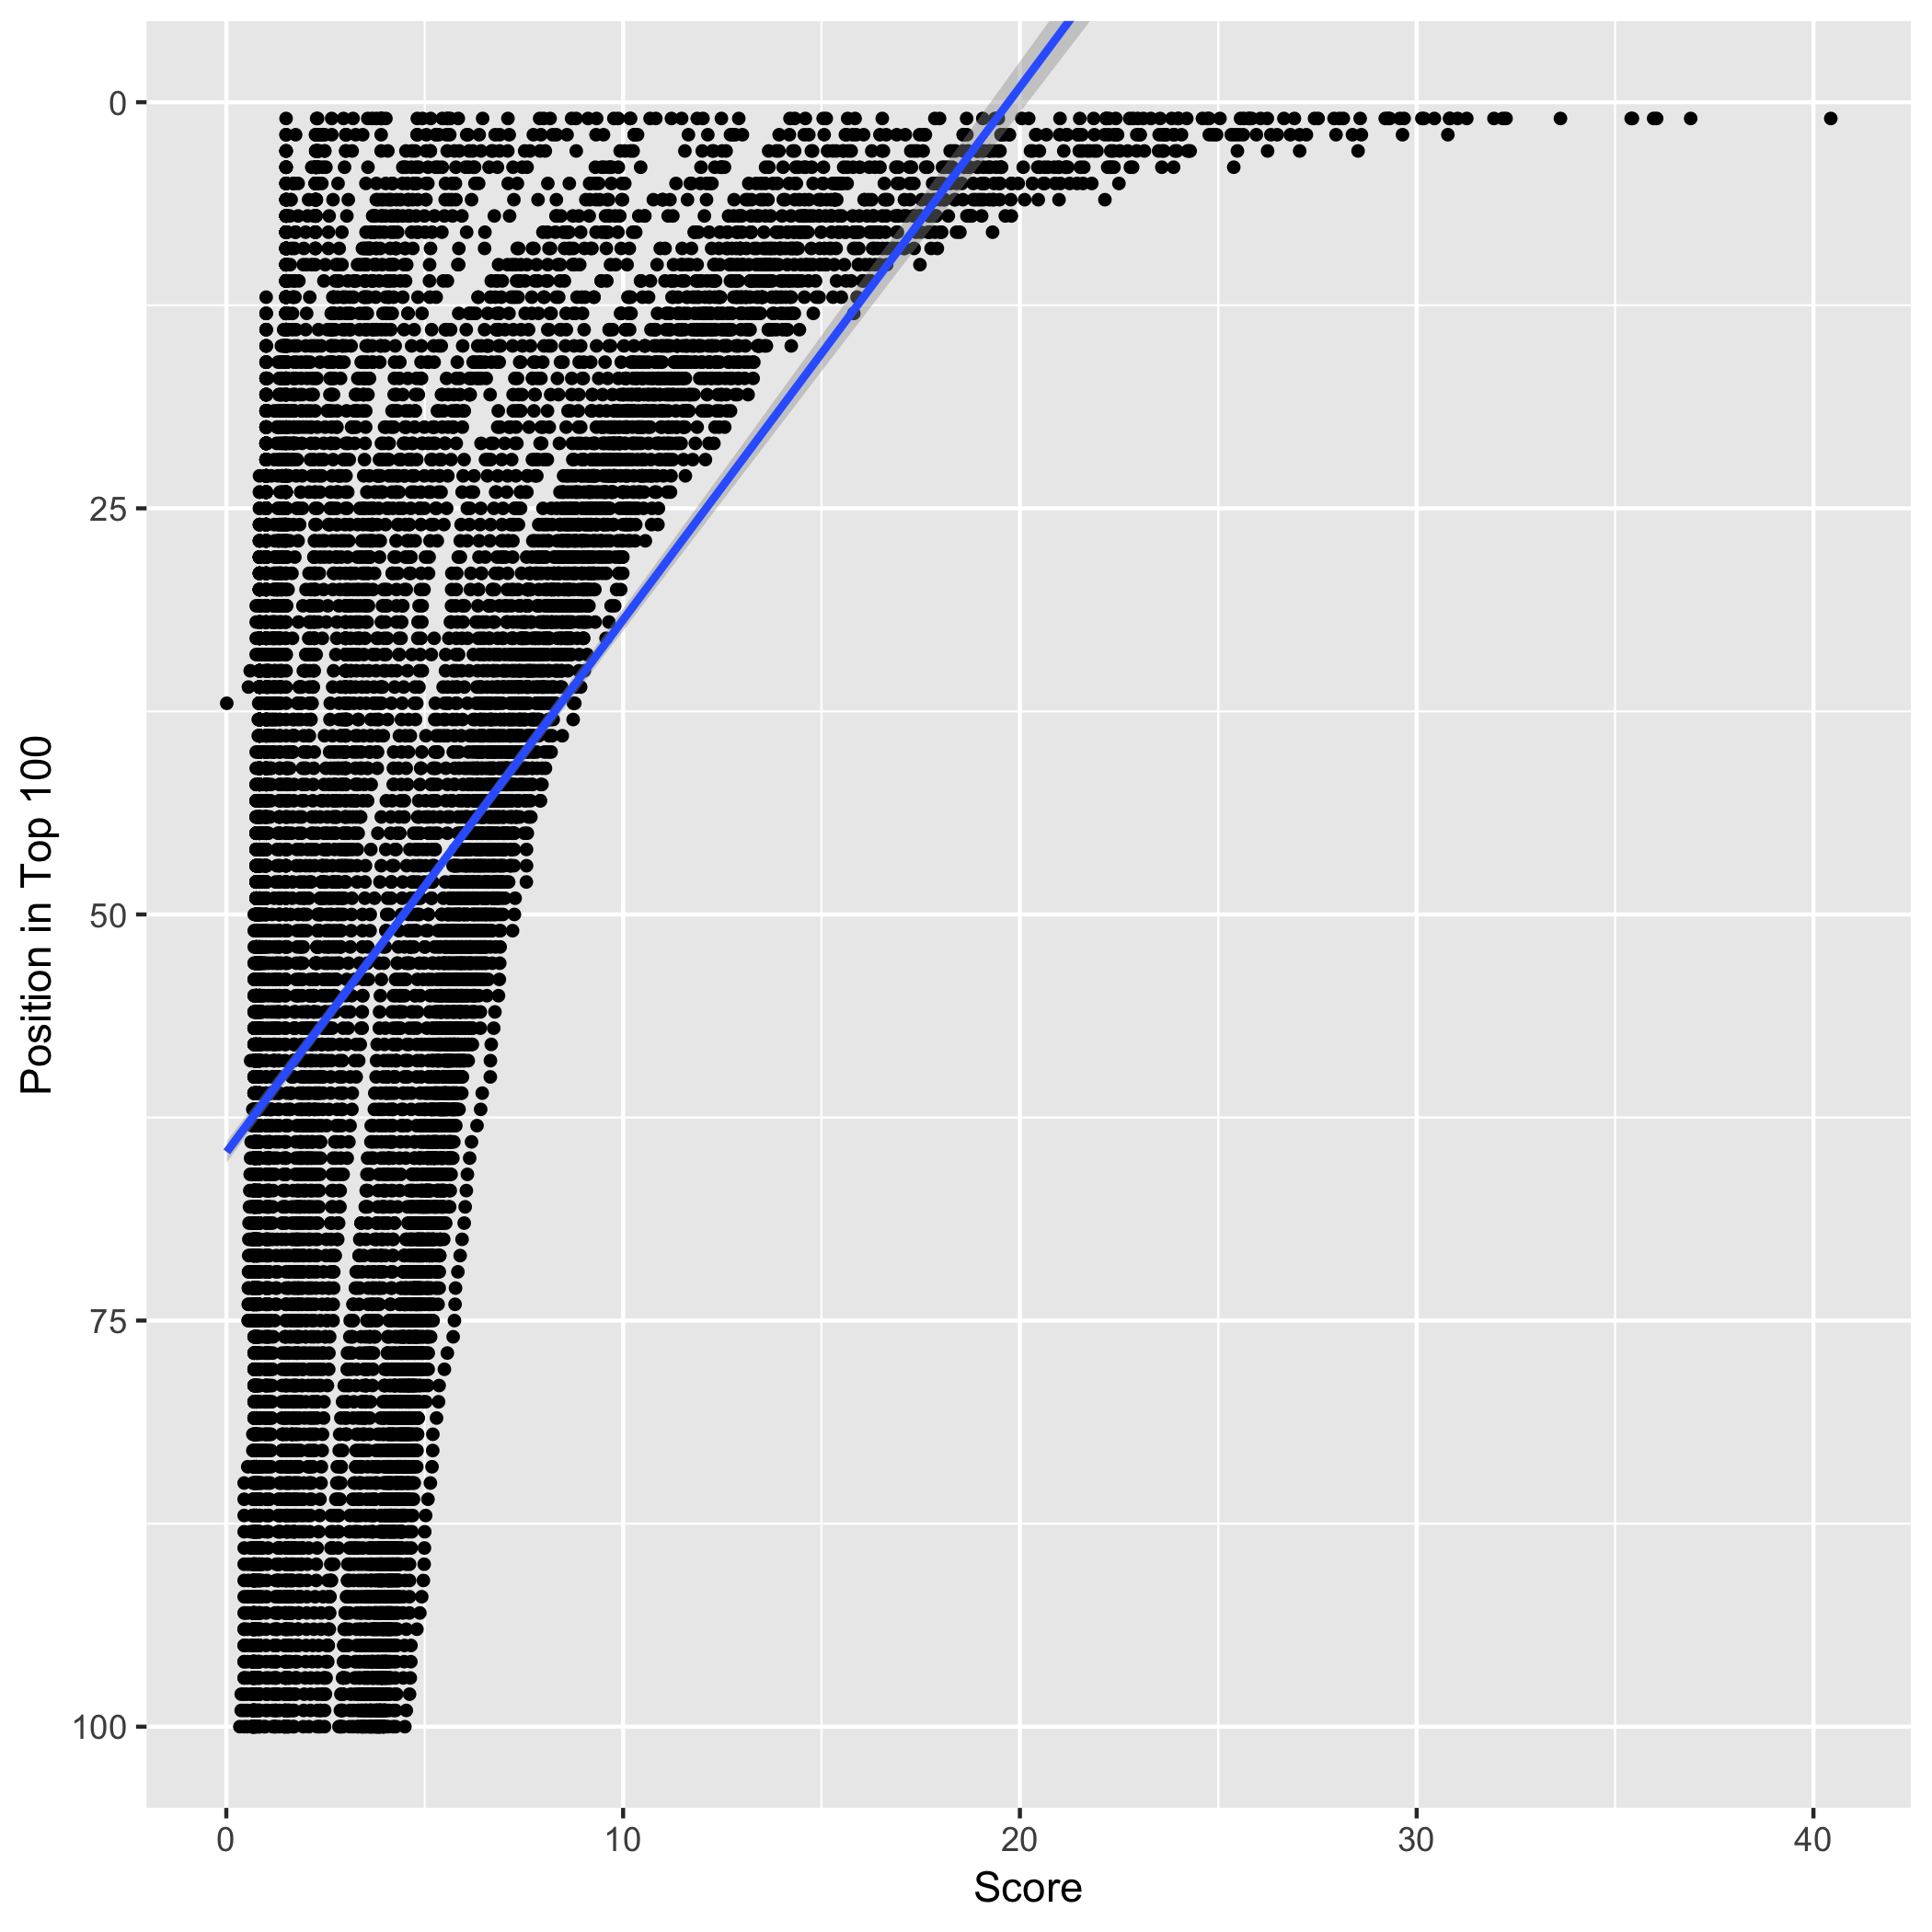
\includegraphics[width=0.5\textwidth]{scoreSell}
          \label{fig:q2}
\end{SCfigure}
        In Figure \ref{fig:q2} we see that again the line of best fit follows an upward trend, however many of the songs are of very low scores indeed.
        It may be worth looking at these on a year-by-year basis, similar to the previous graph, however for the moment it is reasonable to conclude that if a song is more highly rated by critics it will also sell better.

\subsection{What is the change in ratio between singles and albums released over the years?}
        A coloured line graph should be used for this visualisation the data is trivariate and 2 of those variables are continuous.
        A large amount of manipulation had to be done to the data here, creating a new dataframe with only the year and type of music.
        That dataframe was then spread
        \myfig
          \caption{Line graph to show year against numbers of albums and singles}
          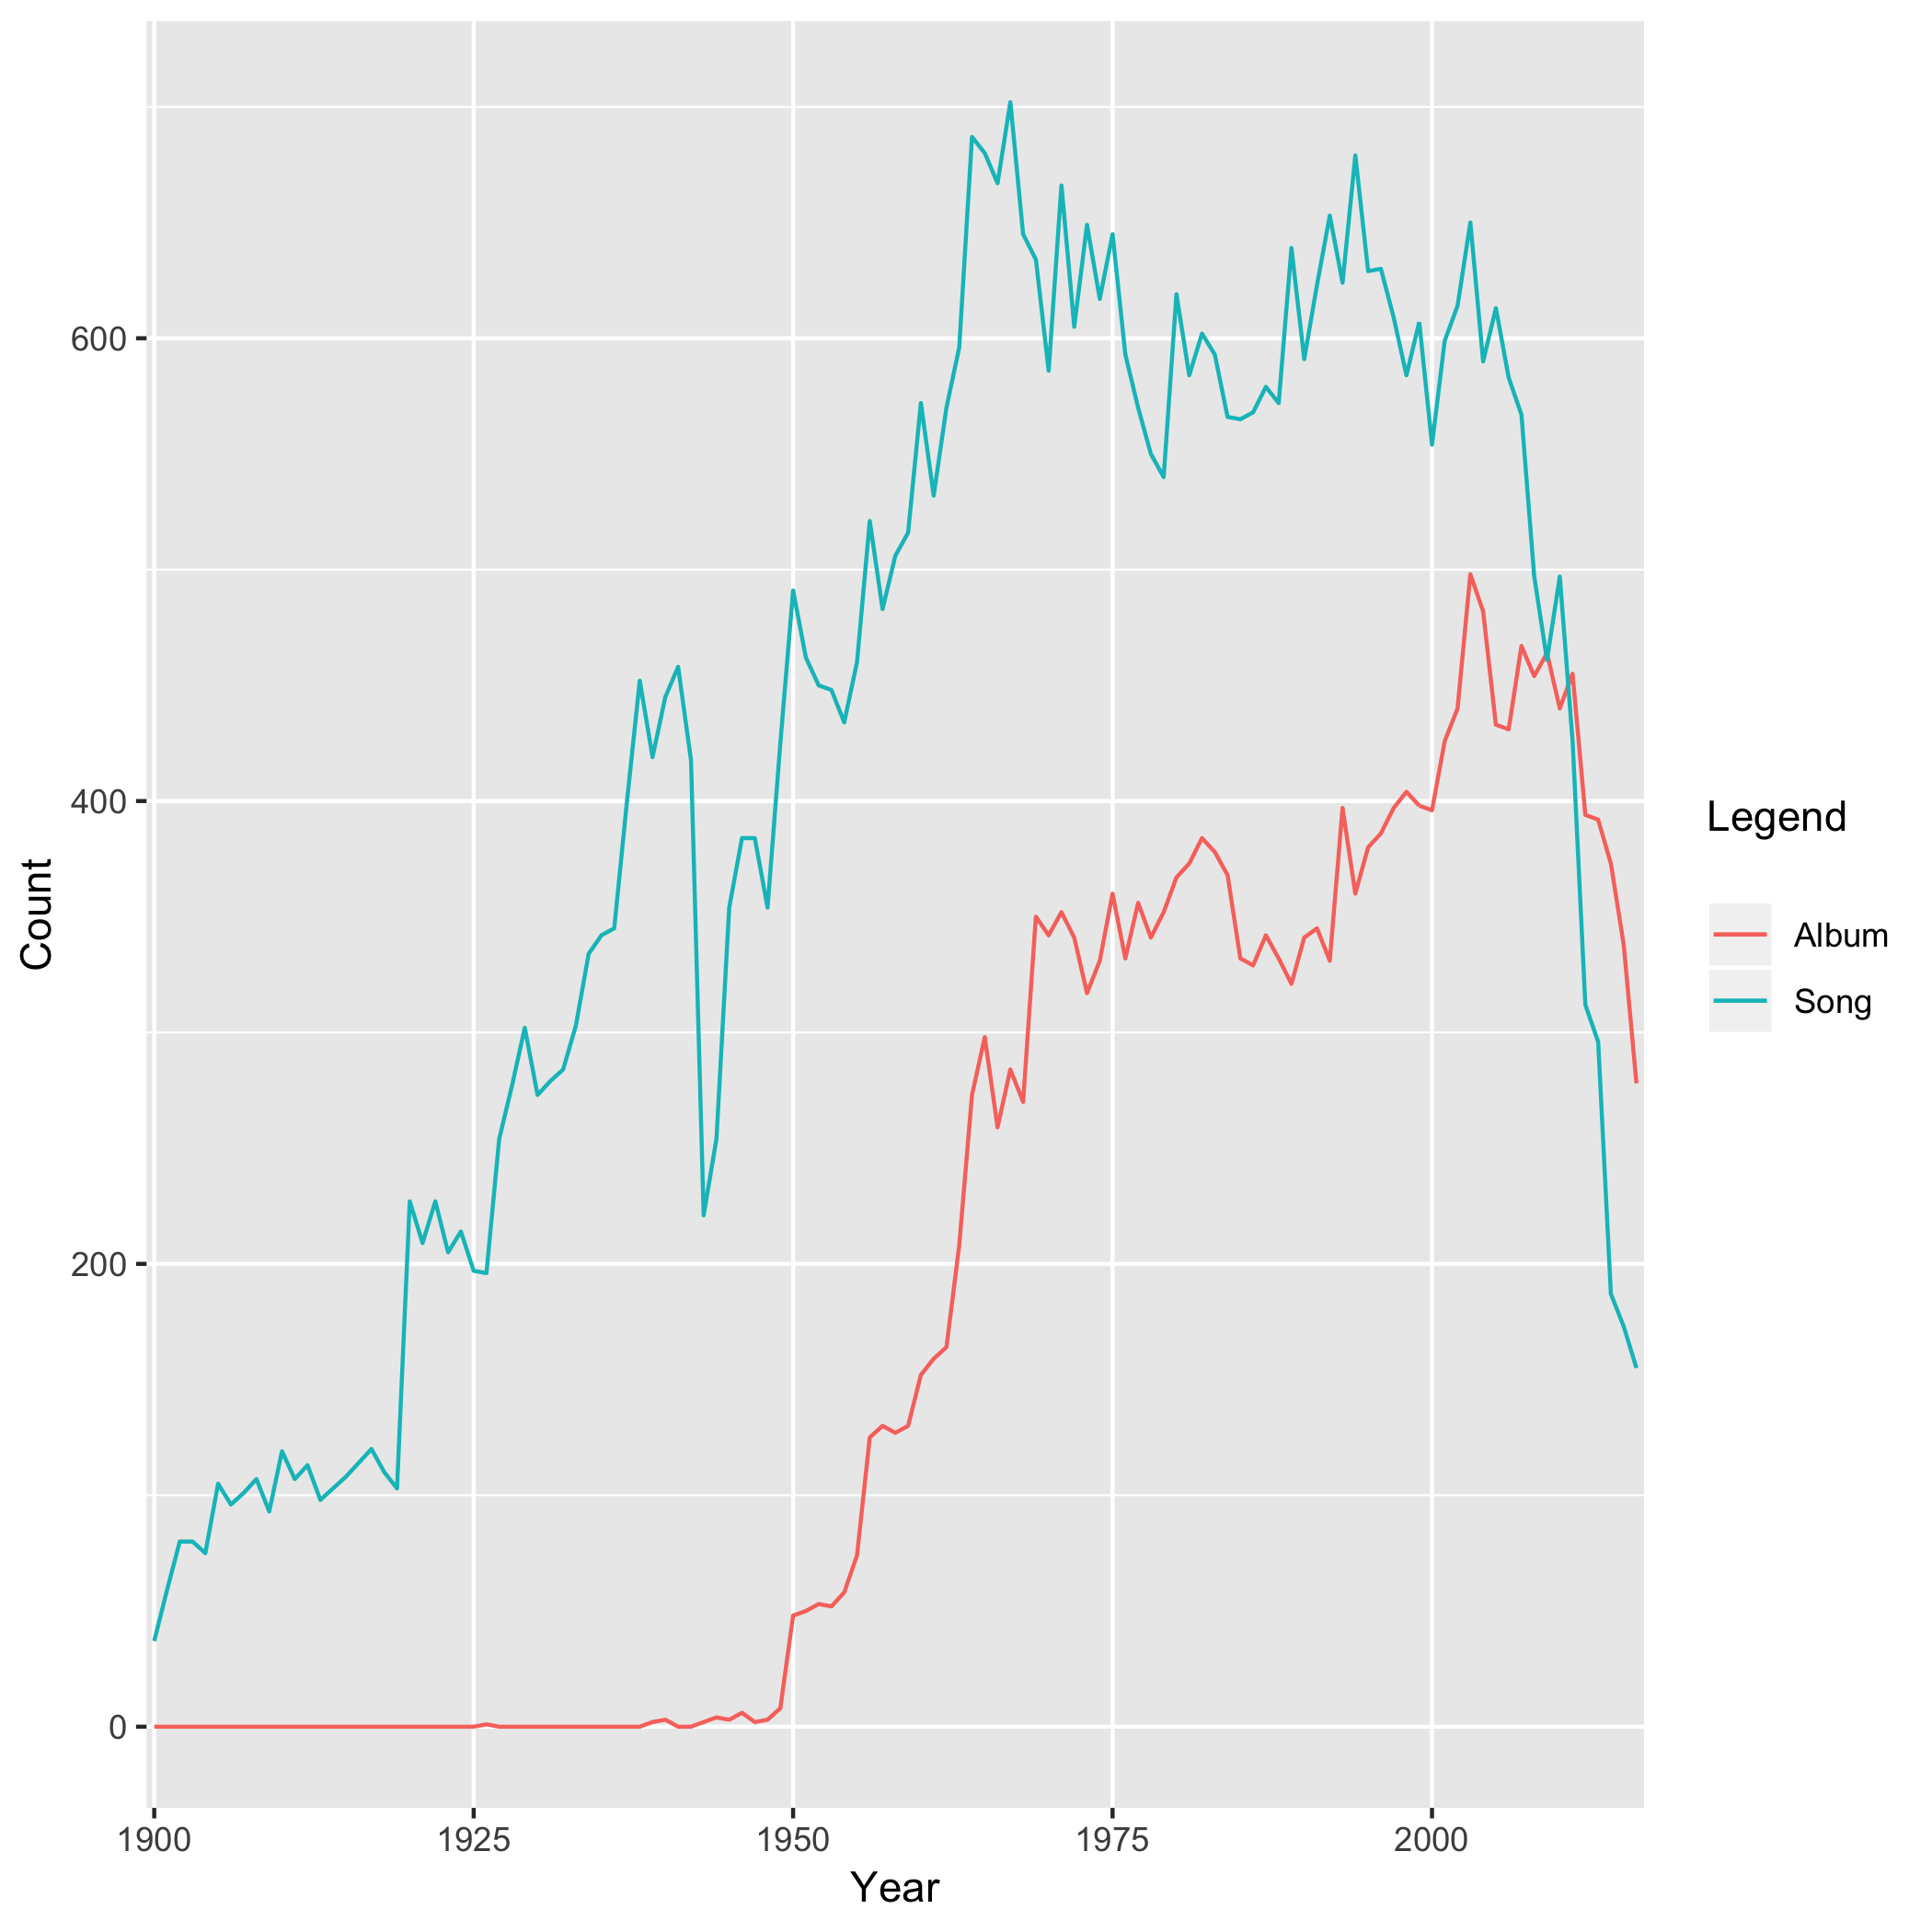
\includegraphics[width=0.5\textwidth]{singlesAlbums}
          \label{fig:q3}
        \end{SCfigure}
        Based on the data in Figure \ref{fig:q3}, we can see that there have consistently been more albums available that singles.
        This is an interesting result, as one would tend to assume that multiple singles can come from one album and that consequently could skew the data.
        However, in the past few years, more singles are being made available, with album figures dropping dramatically.

\pagebreak

\section{New Questions \& Further Visualisations}
    \subsection{Does a song's position on the top 100 of the year affect its position on the top 100 of the decade?}
        It stands to reason that this should be the case; if a song sells more in a year it should sell more over the decade, however there may have been more overall records sold in different years, and a song that was number one for one year may not have broken the top 10 of another.
        This information can be plotted by a simple scatter graph, alongside a line of best fit.

        \myfig
          \caption{Scatter graph showing top 100 of the year positions of all decades number 1 selling song}
          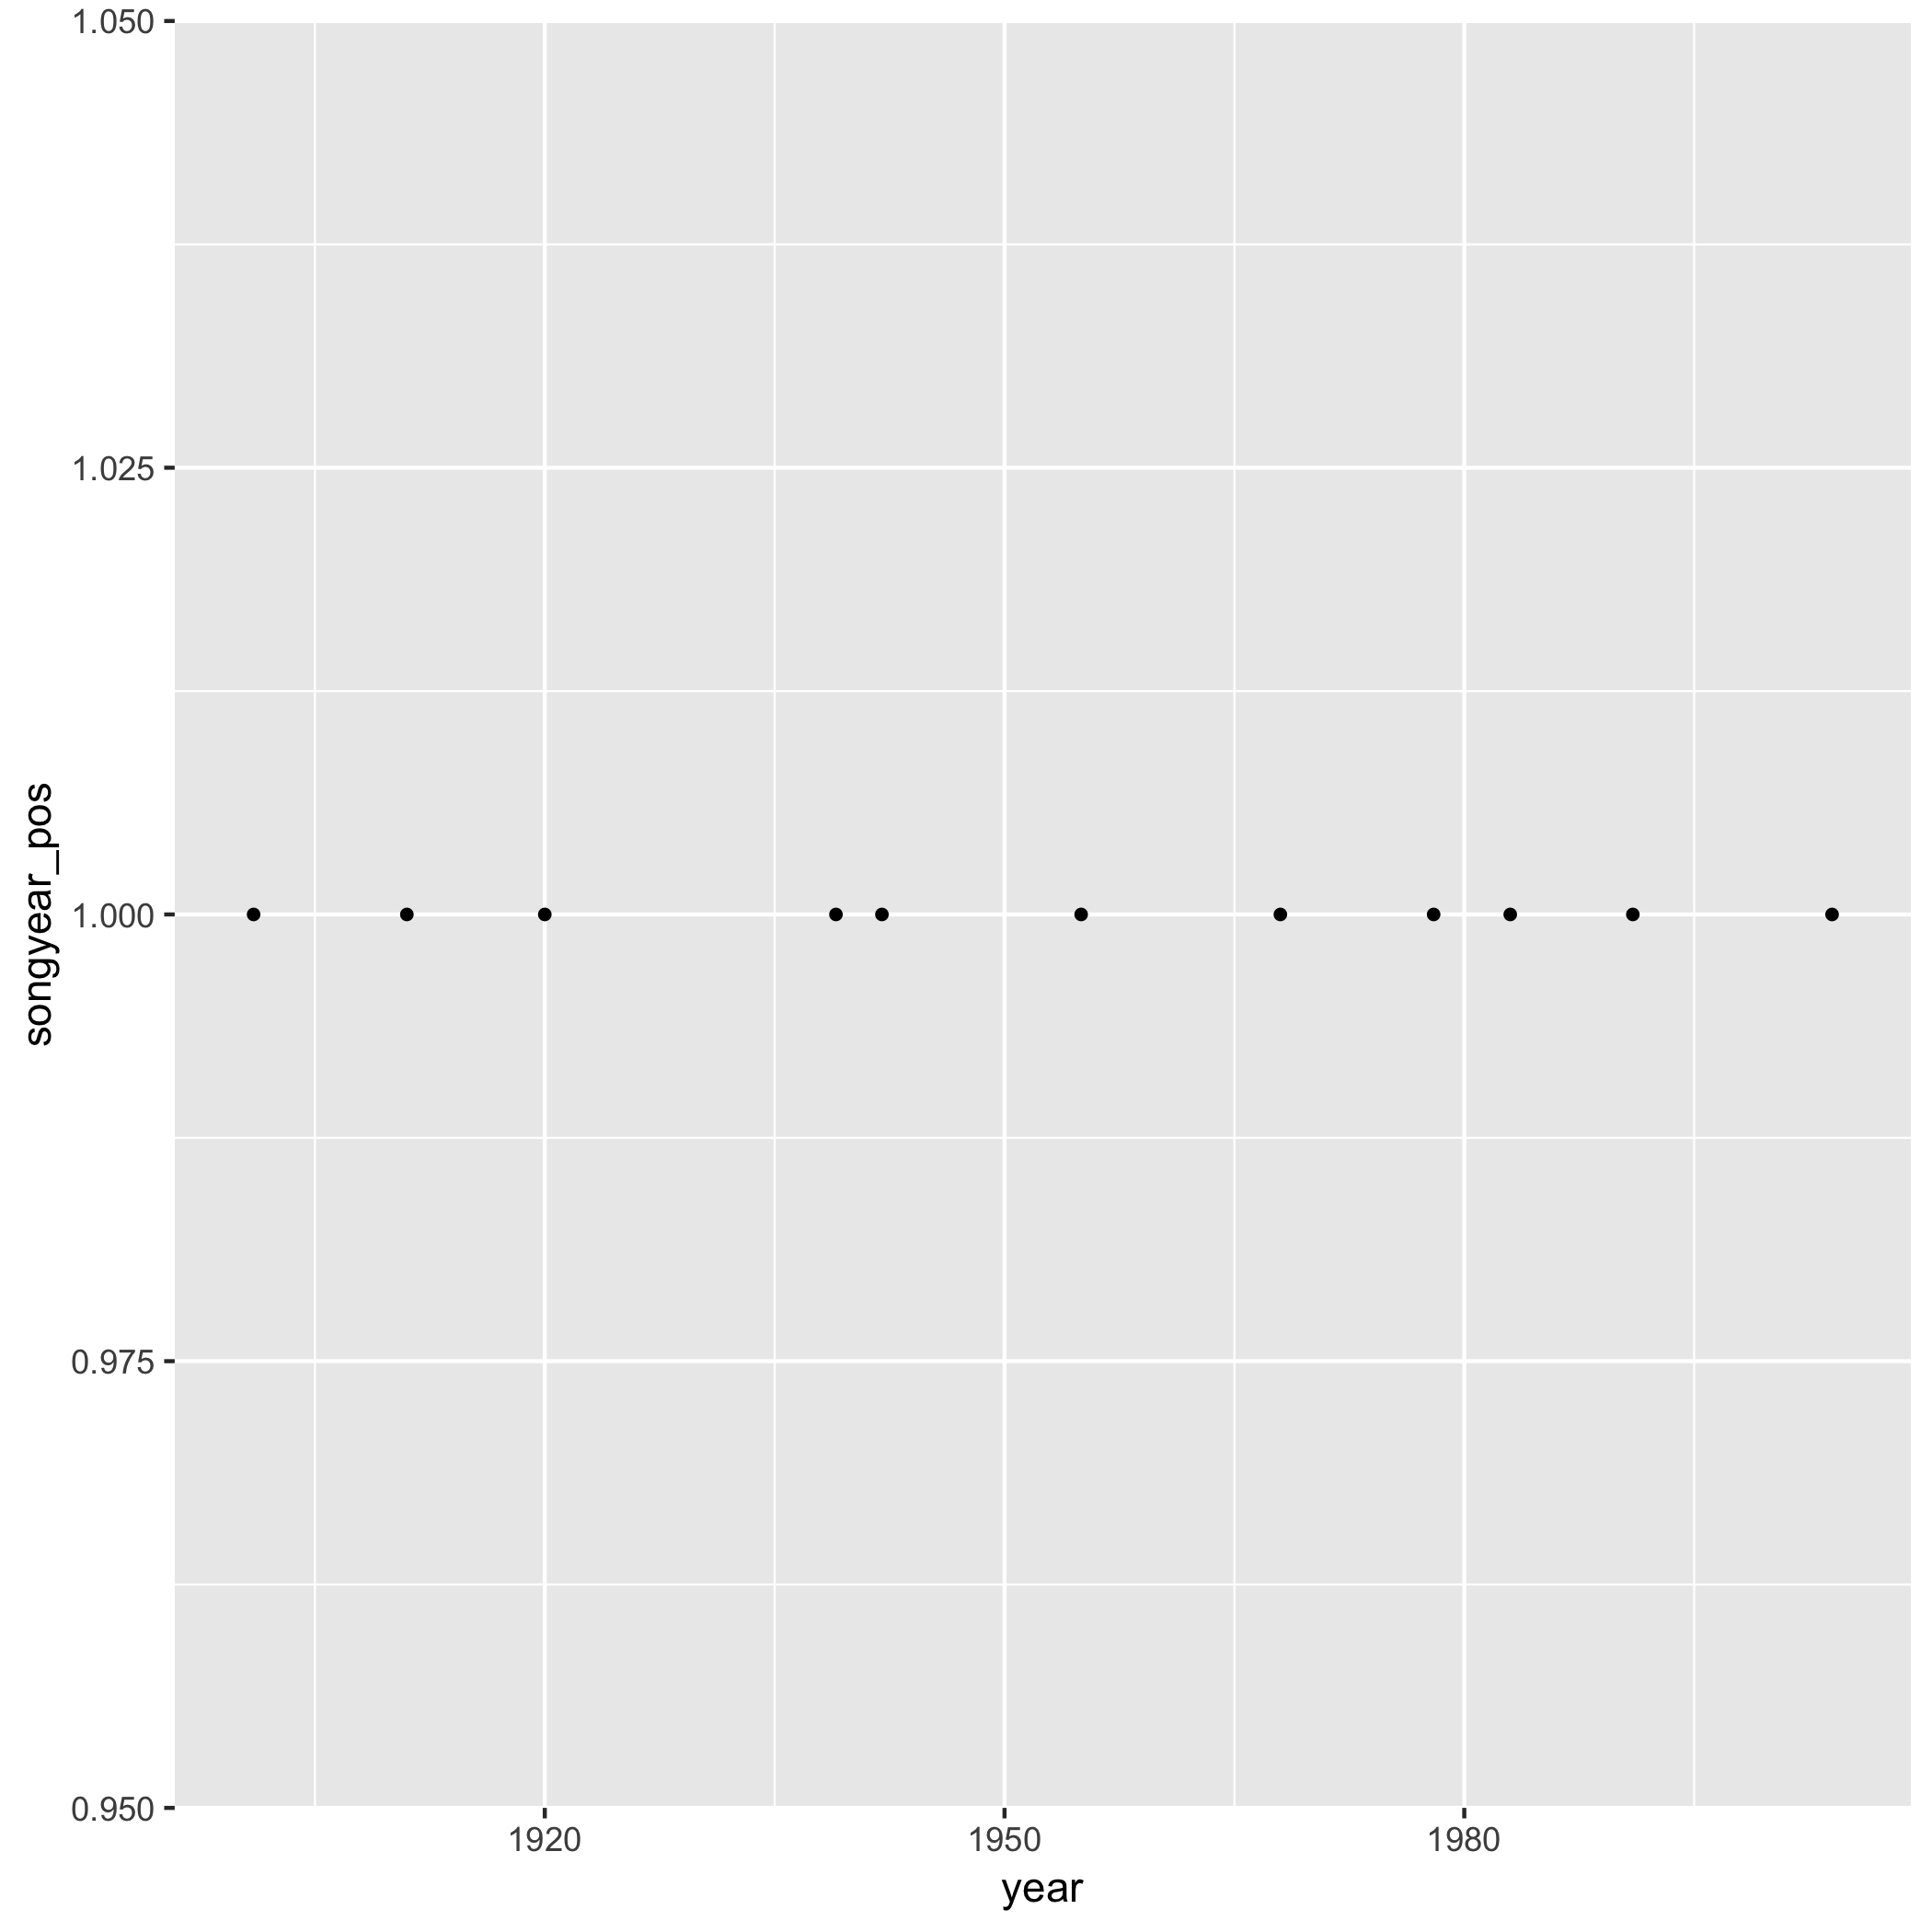
\includegraphics[width=0.5\textwidth]{topSell}
          \label{fig:q4p1}
        \end{SCfigure}

        \myfig
          \caption{Scatter graph showing the overall relation between position on top 100 of the year and top 100 of the decade}
          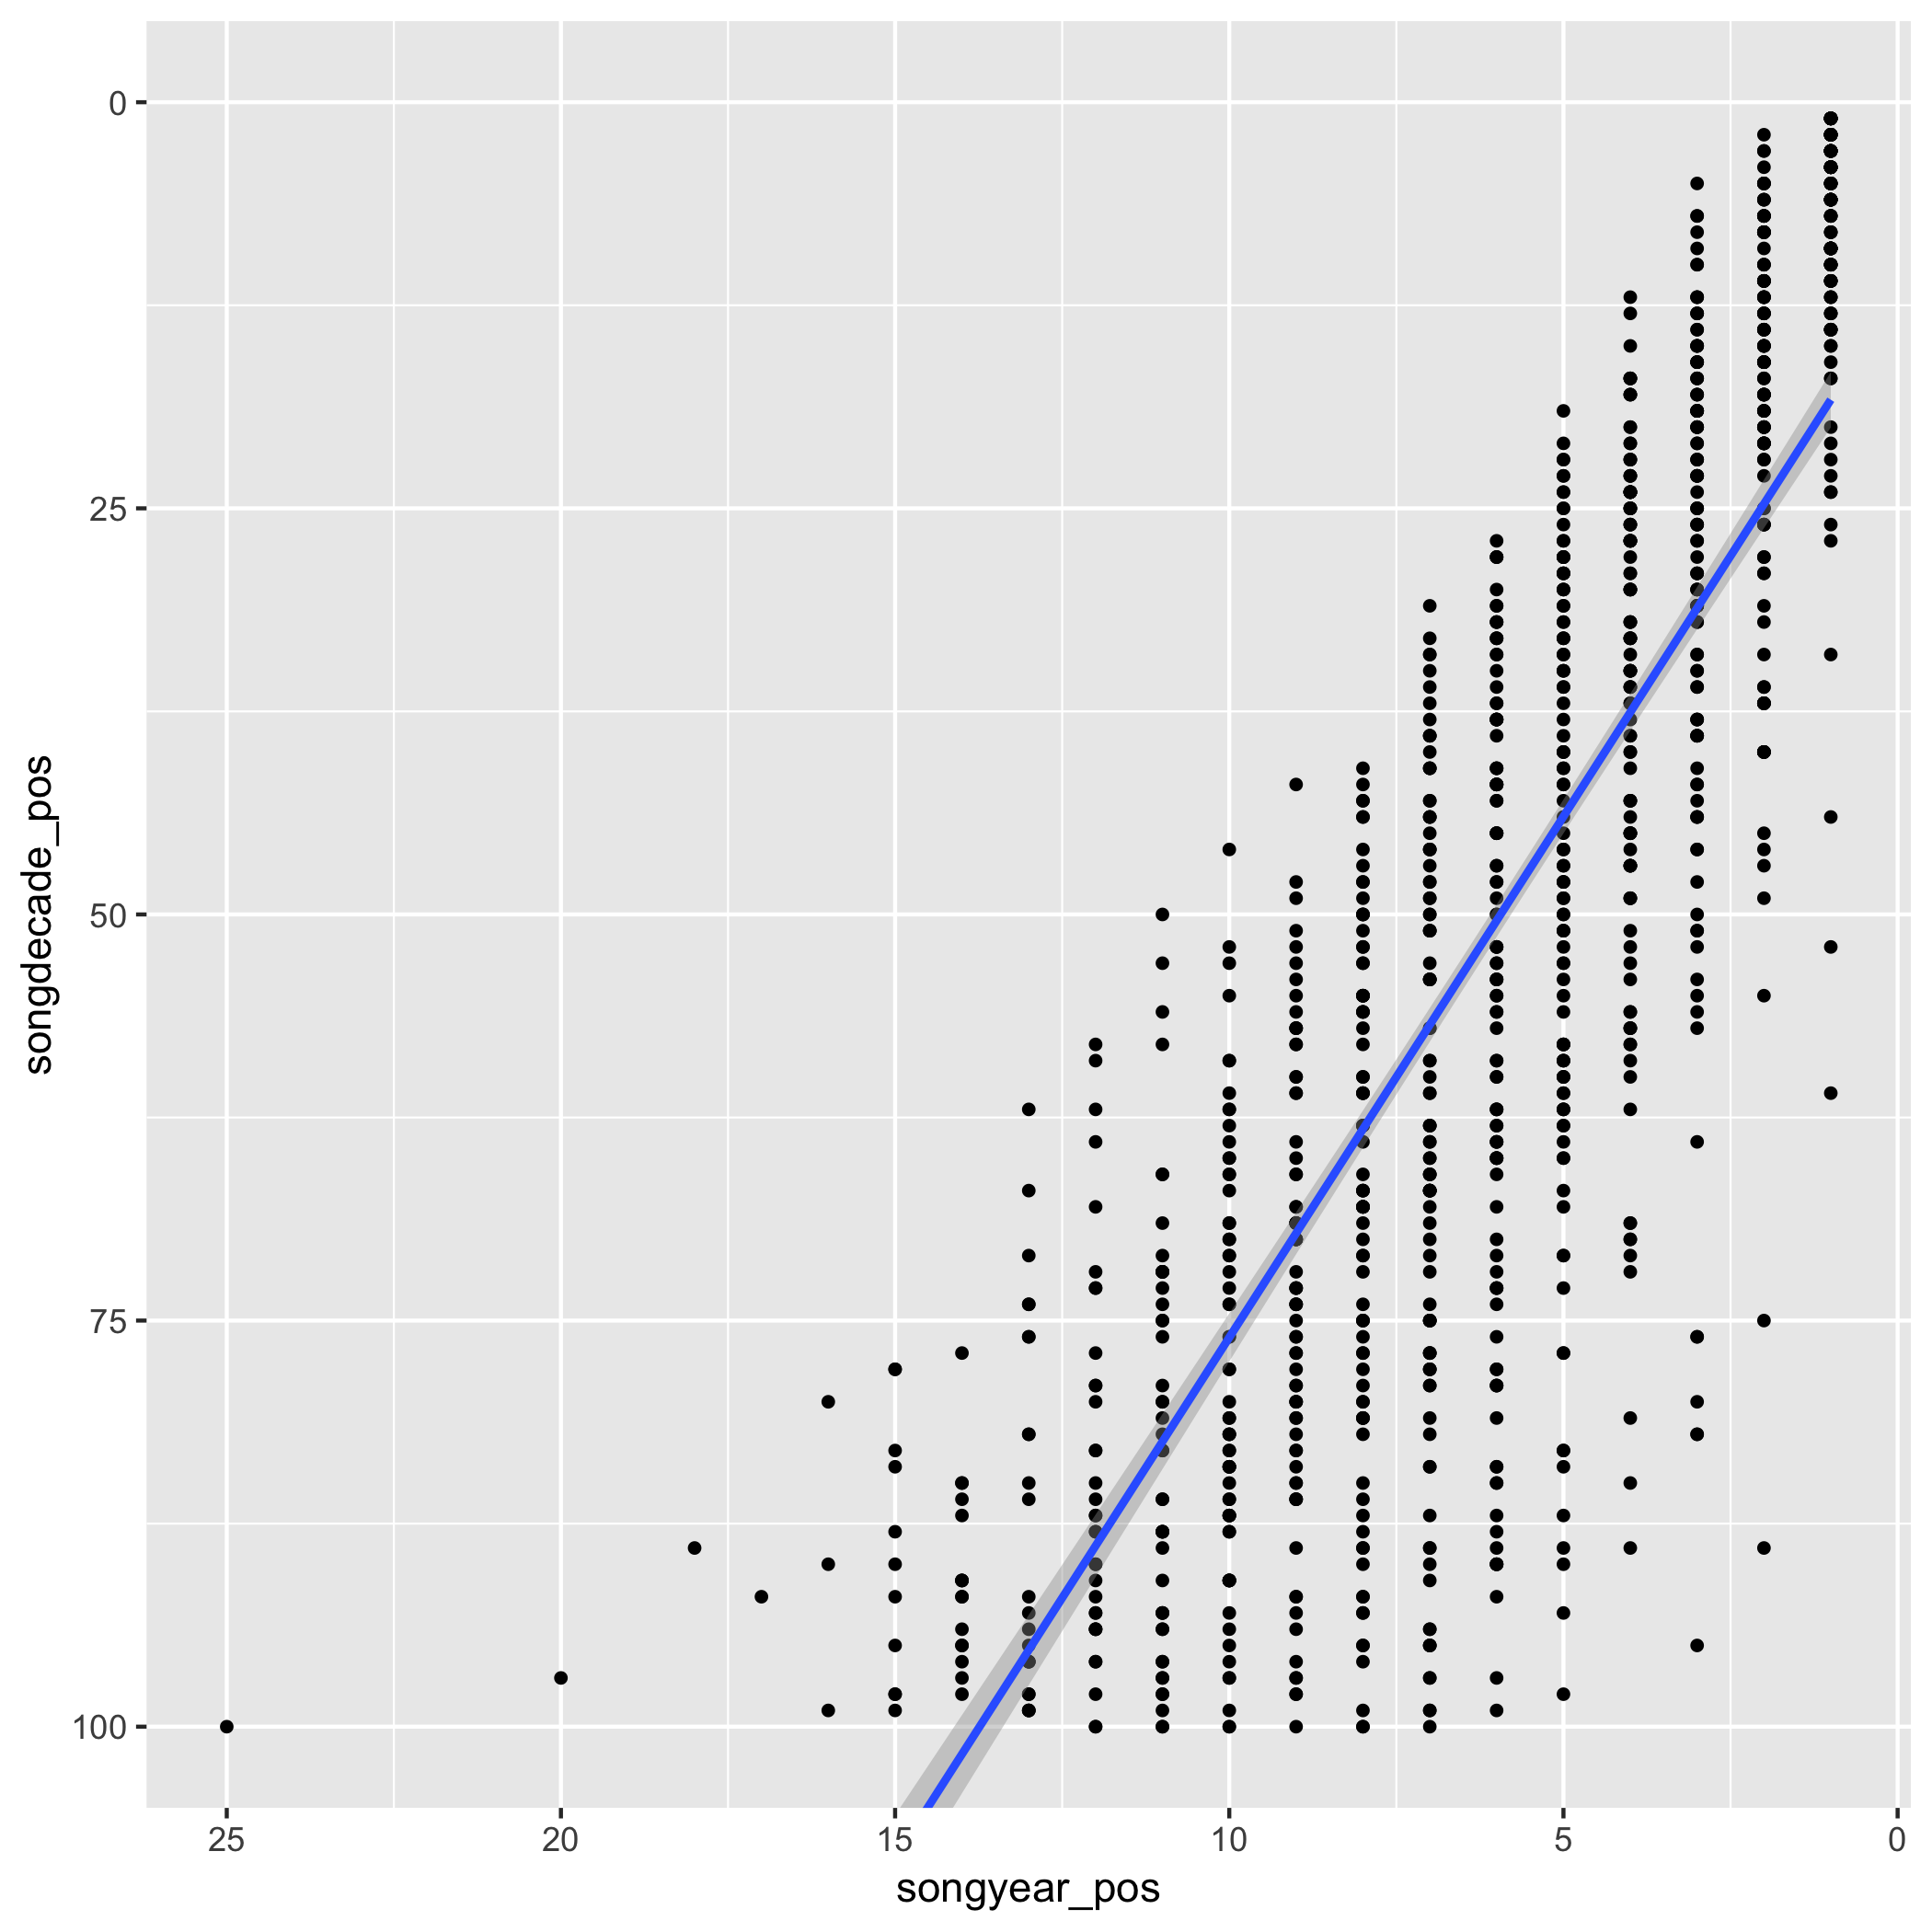
\includegraphics[width=0.5\textwidth]{yearDecade}
          \label{fig:q4p2}
        \end{SCfigure}

        The graph in Figure \ref{fig:q4p1} is to show that every decade's number one selling song was also the top-selling song of its year.
        This is to help put Figure \ref{fig:q4p2} into more context, especially at the higher end of both axes.
        From this we can see that there is a general trend that songs that do better in their respective years also do better in the decade charts.
        It is also interesting to note that the lowest \verb|songdecade_pos| of any top 100 decade song is 25.
        If this was evenly distributed it should be the top 10s of every year, however clearly this is not the case.

        \myfig
          \caption{Scatter graph showing year chart positions of every decade's top 100 song against year}
          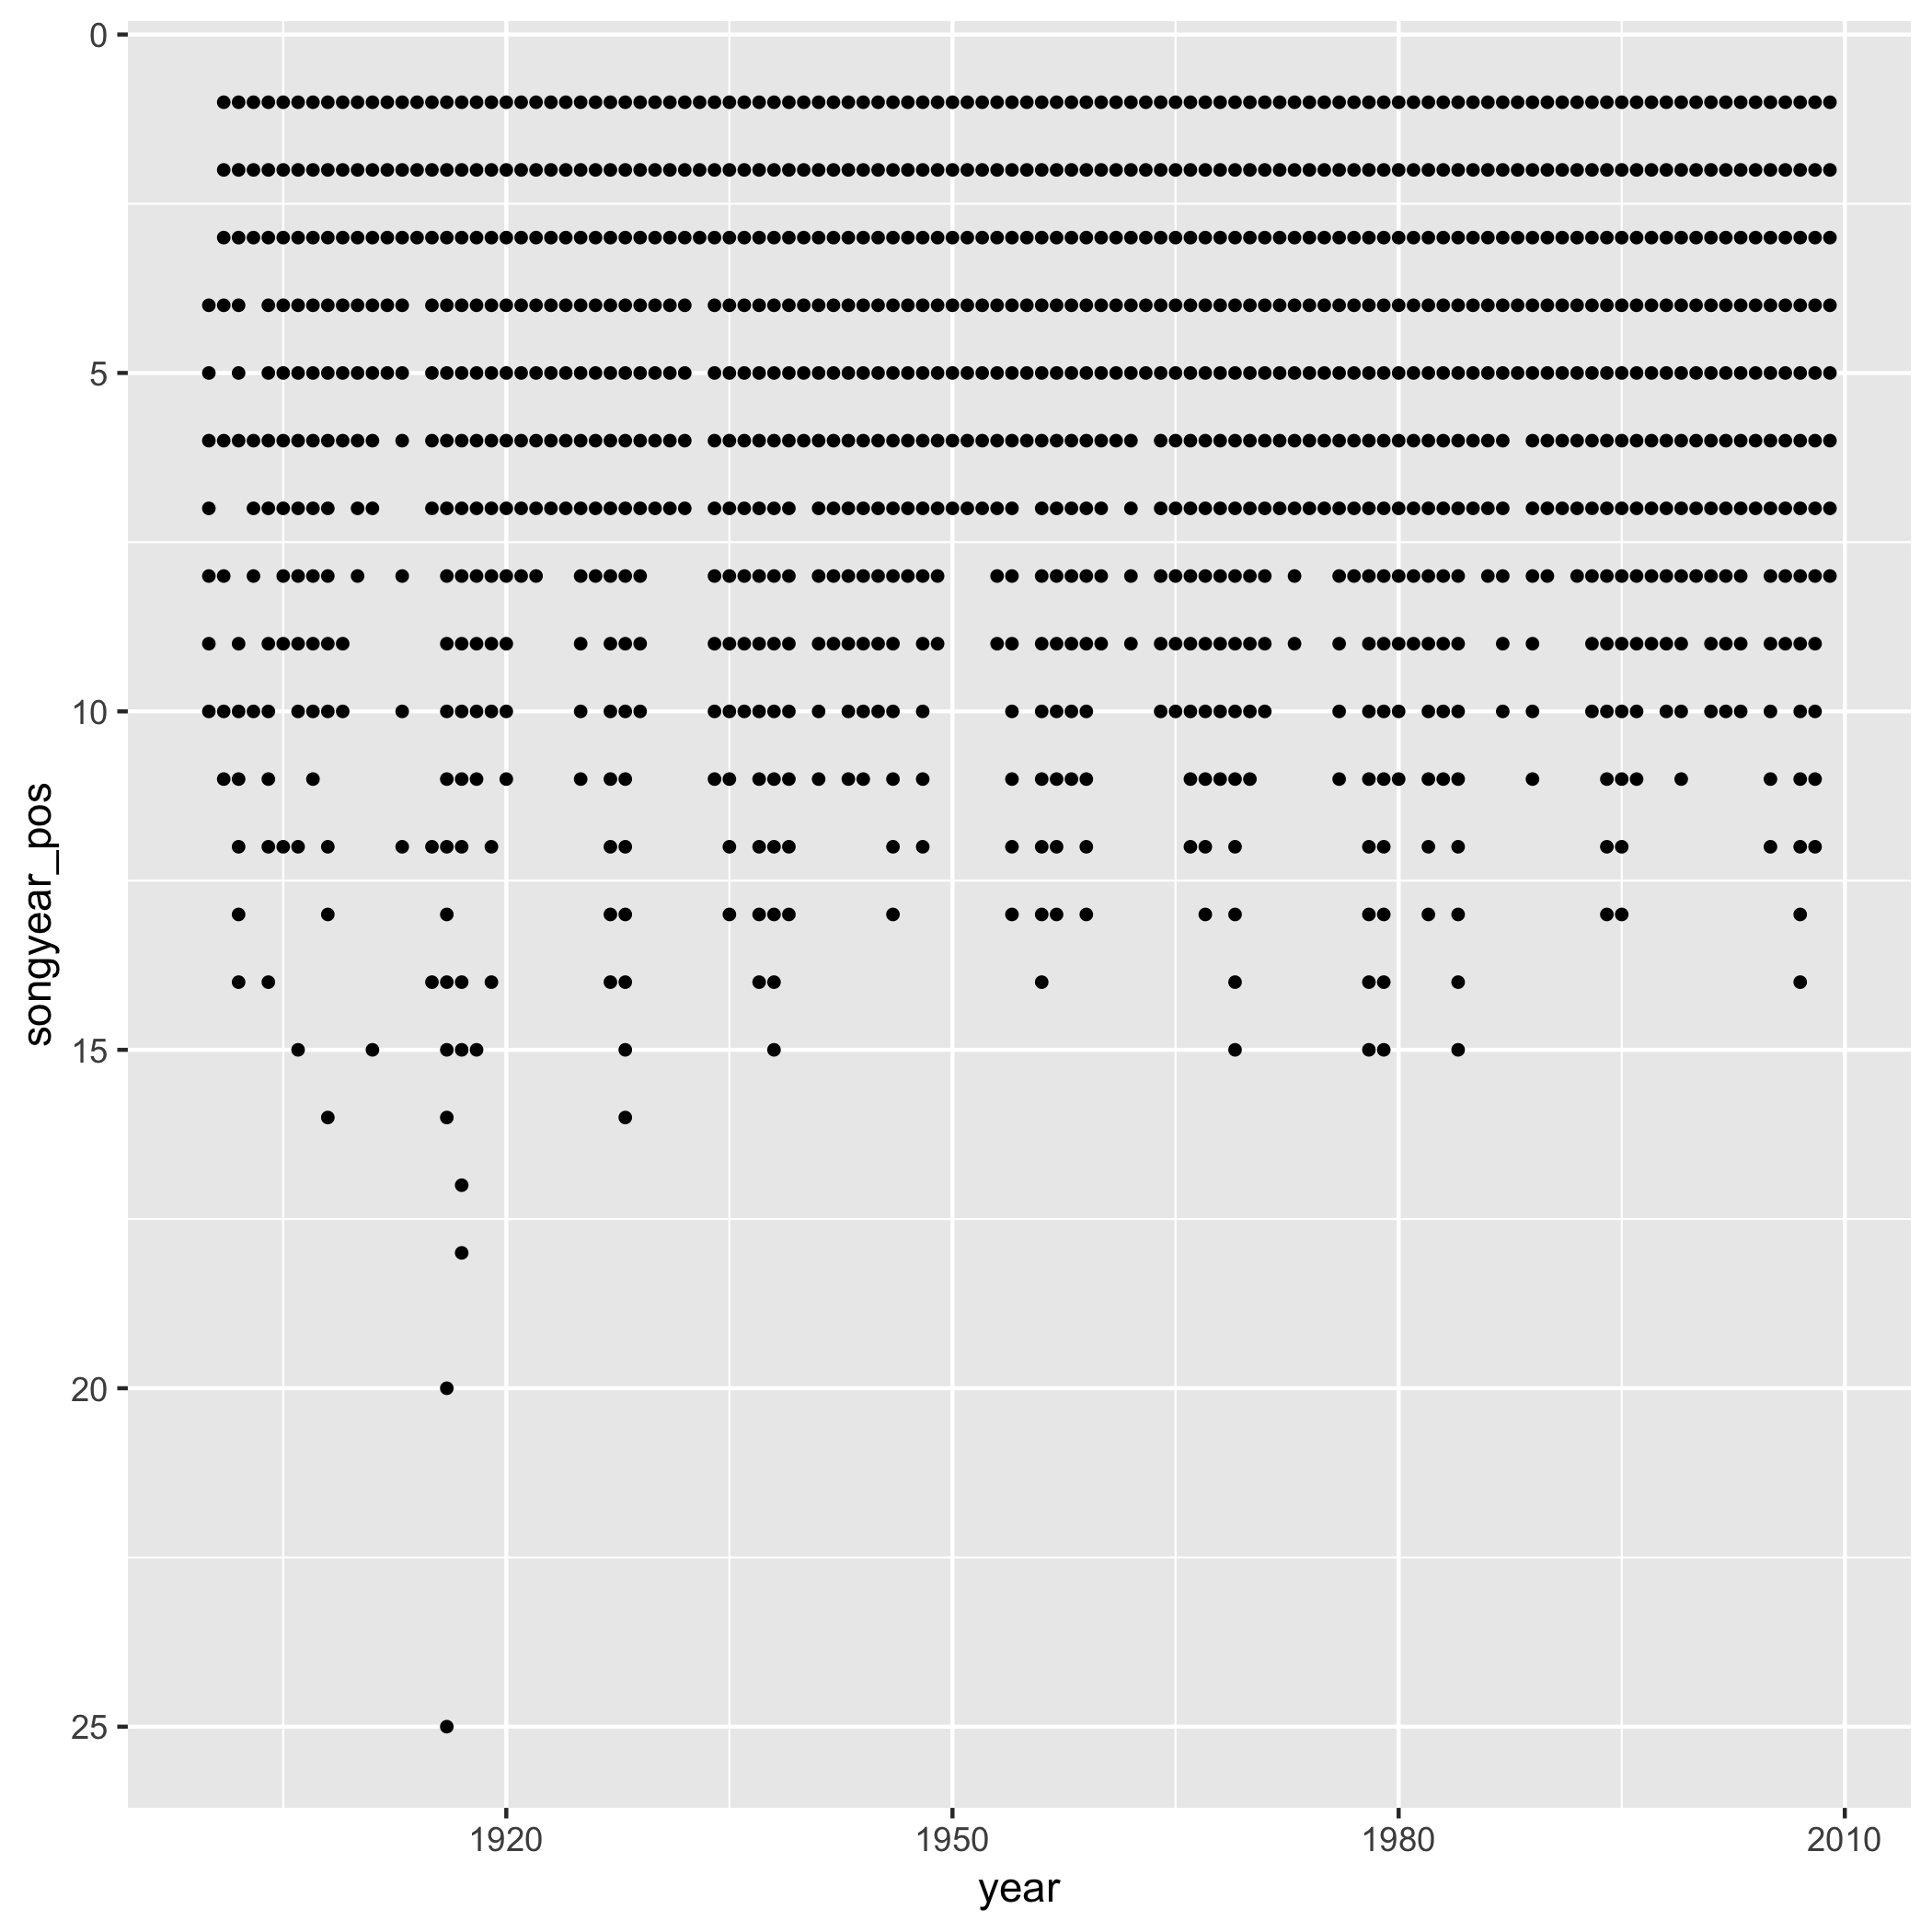
\includegraphics[width=0.5\textwidth]{yearDecade2}
          \label{fig:q4p3}
        \end{SCfigure}

        From Figure \ref{fig:q4p3} we can see that some time around 1918 there was a boom in record sales, as the 25th best selling record of that year wound up on the decade's top 100, compared to 1916 where only up to number 3 made it onto the decade chart.
        We can likely surmise that this is due to WWI taking away demand for music, and the end of the war bringing about a time of celebration and a boom to the record industry.



    \subsection{If an artist has many top-100 songs, will they also have many top-100 albums?}
        For this we should take the top 25 artists, this is to say the 25 artists with the most representation in the yearly top 100 songs, and see whether or not their representation in the yearly top 100 albums scales proportionally.
        This can be done by way of a 'split' bar chart, with the artists on the y-axis and the number of Top 100 spots taken on x.
        A large amount of data manipulation had to take place here; first a new dataframe was created containing only the artist name and \verb|songyear_pos| and \verb|albumyear_pos| of each row.
        Then this was ordered by artist name such that it could be aggregated, however before this happened the \verb|songyear_pos| and \verb|albumyear_pos| values were modified such that any non-NA value was mapped to 1, and NA values mapped to zero.
        This was done because we are only interested in the number of Top 100 songs/albums, not their respective positions.
        This resultant dataframe was aggregated, summing the values in the \verb|songyear_pos| and \verb|albumyear_pos| columns based on the artist name.
        This was then sorted backwards with respect to \verb|songyear_pos| such that the top 25 of this could be taken via head.
        Now we have the top 25 artists with the most Top 100 Songs.
        \myfig
          \caption{Bar Chart to show relation between number of Top 100 Songs and Top 100 Albums of the year per Artist}
          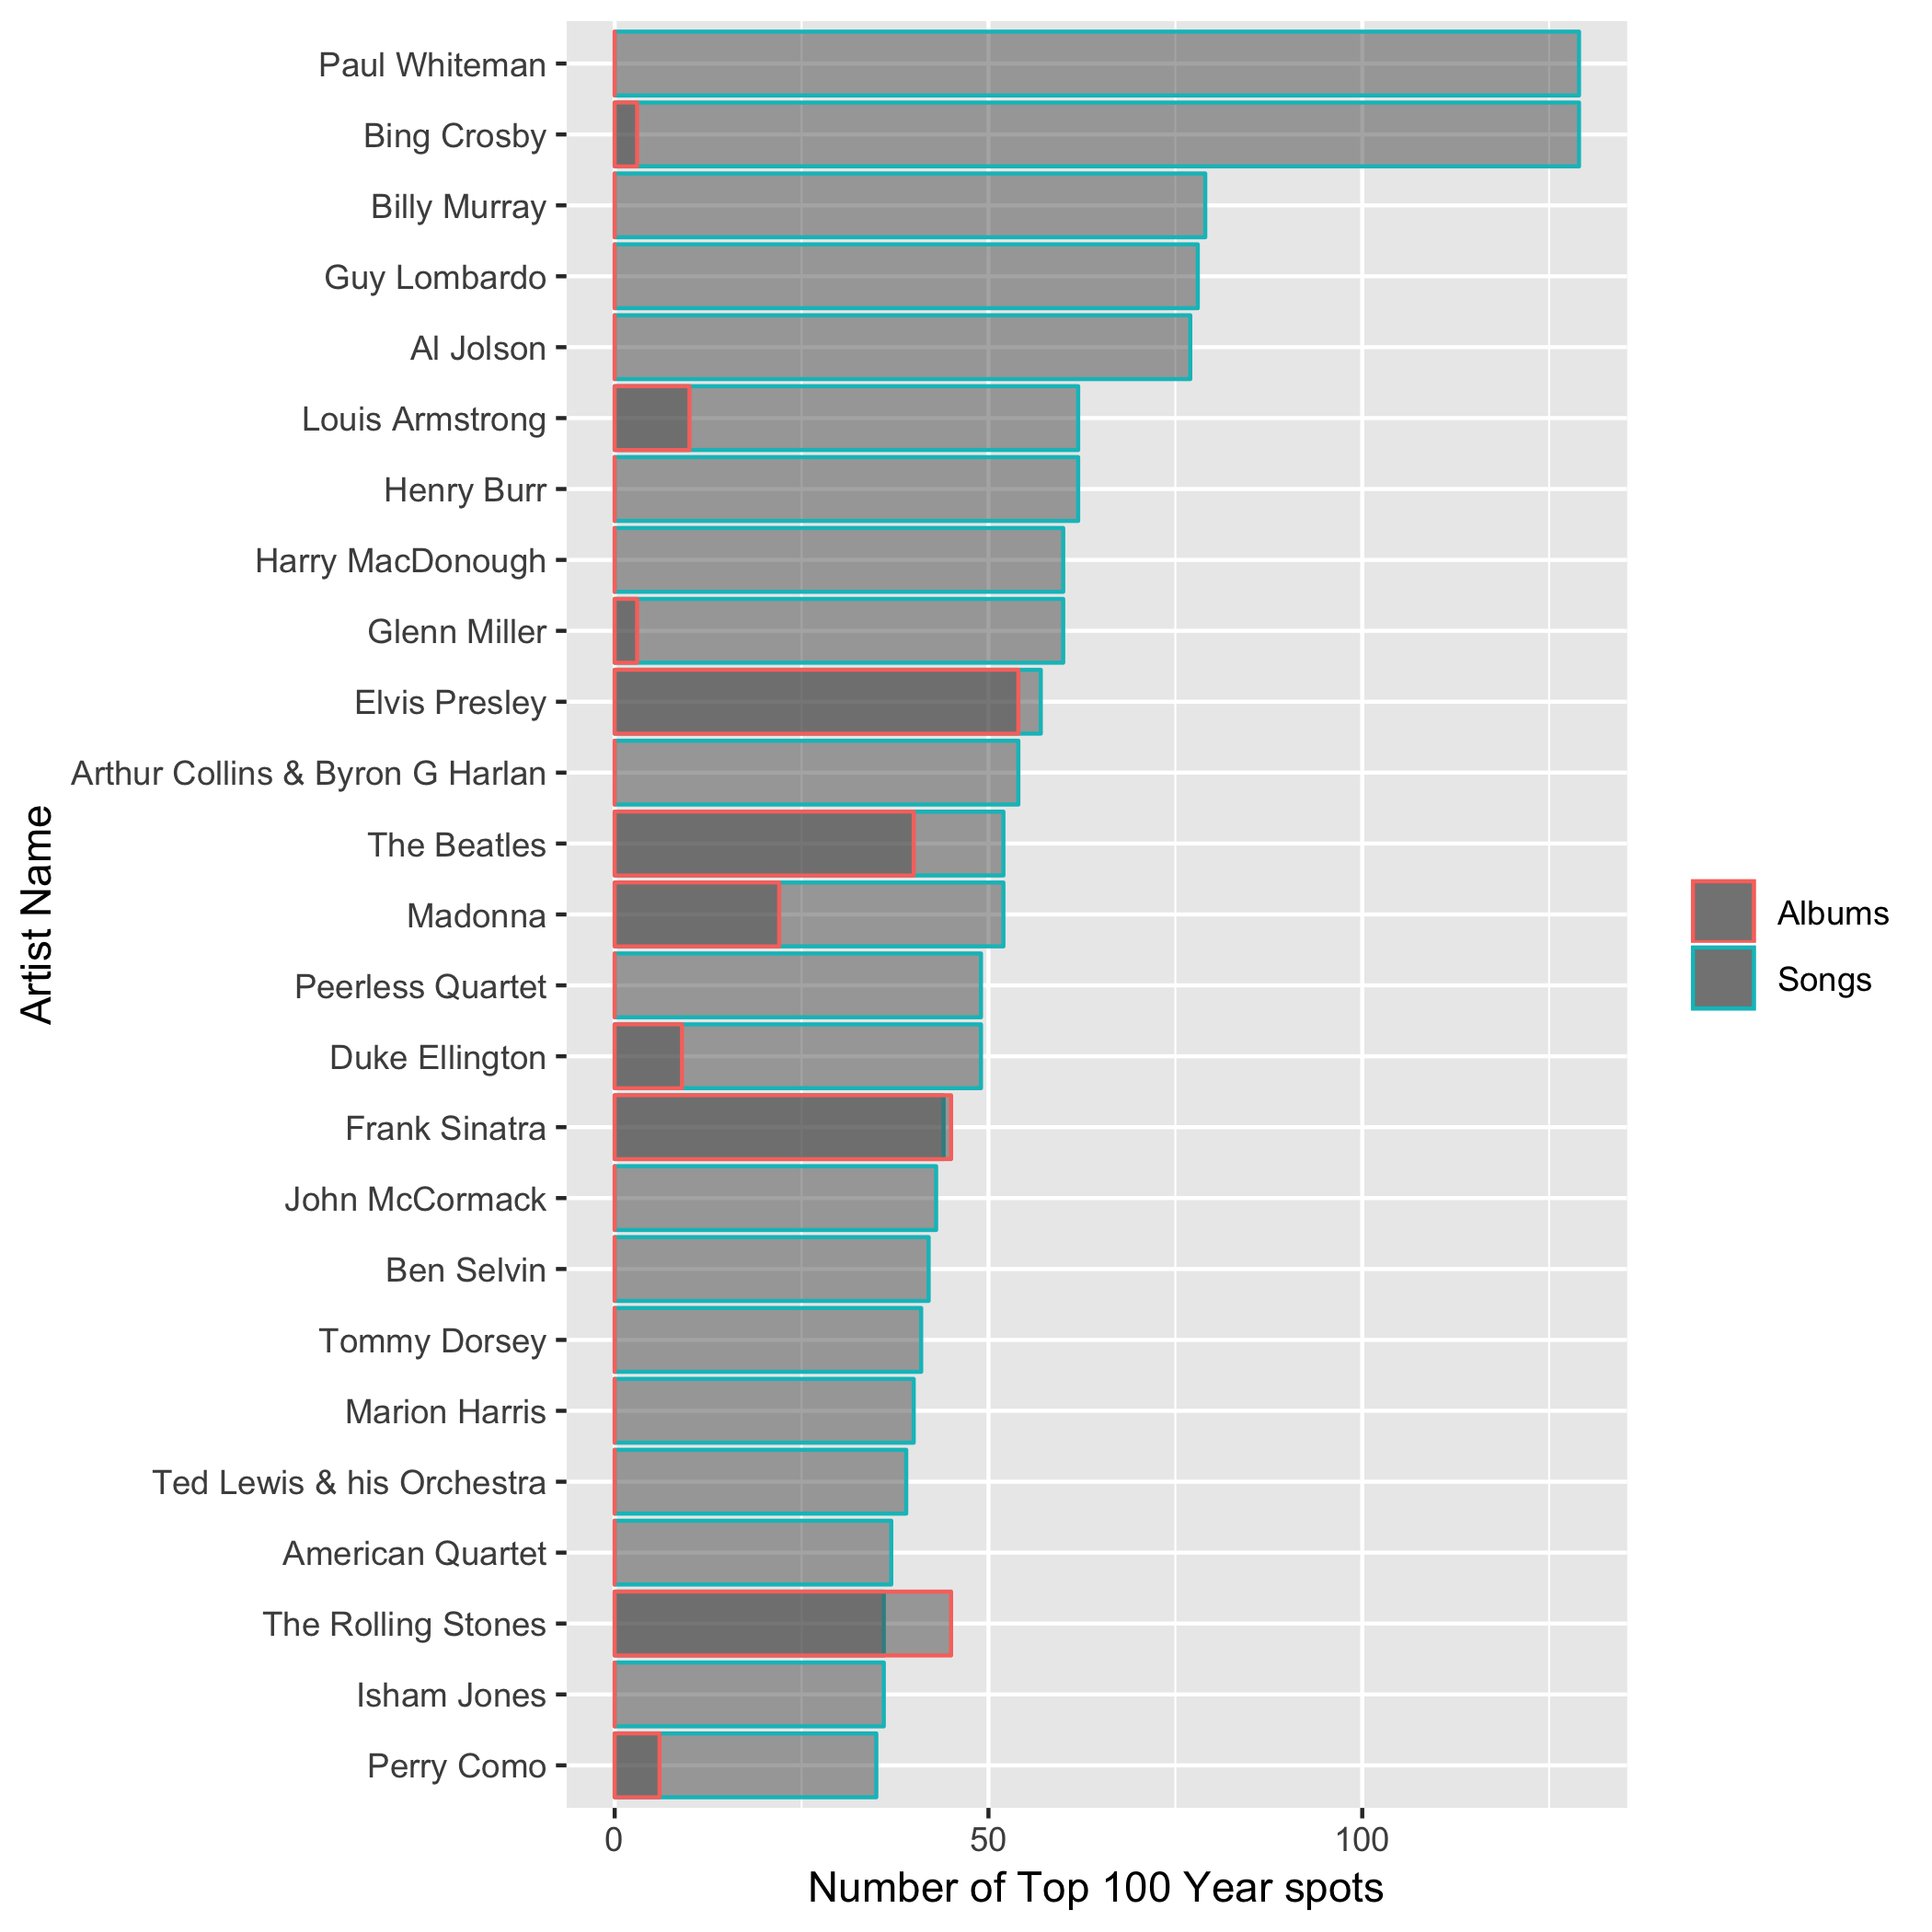
\includegraphics[width=0.5\textwidth]{songAlbum}
          \label{fig:q5}
        \end{SCfigure}

        From Figure \ref{fig:q5} we can see no particular trend in terms of \verb|albumyear_pos|, with Bing Crosby (the highest \verb|songyear_pos| count) having one of the lowest \verb|albumyear_pos| counts.

    \subsection{Are albums usually rated higher than songs?}
        We can determine this on a year-by-year basis, with a visualisation similar to the used in Figure \ref{fig:q3}, only this time plotting mean album scores against mean song scores.
        In terms of data manipulation, I split the main music dataframe into two subframes, one only containing albums and one songs.
        For both of these I aggregated by year, finding the mean scores for each year, and then vertically joined both dataframes to form the basis of the plot.
        \myfig
          \caption{Line Chart showing average ratings for albums and singles against year}
          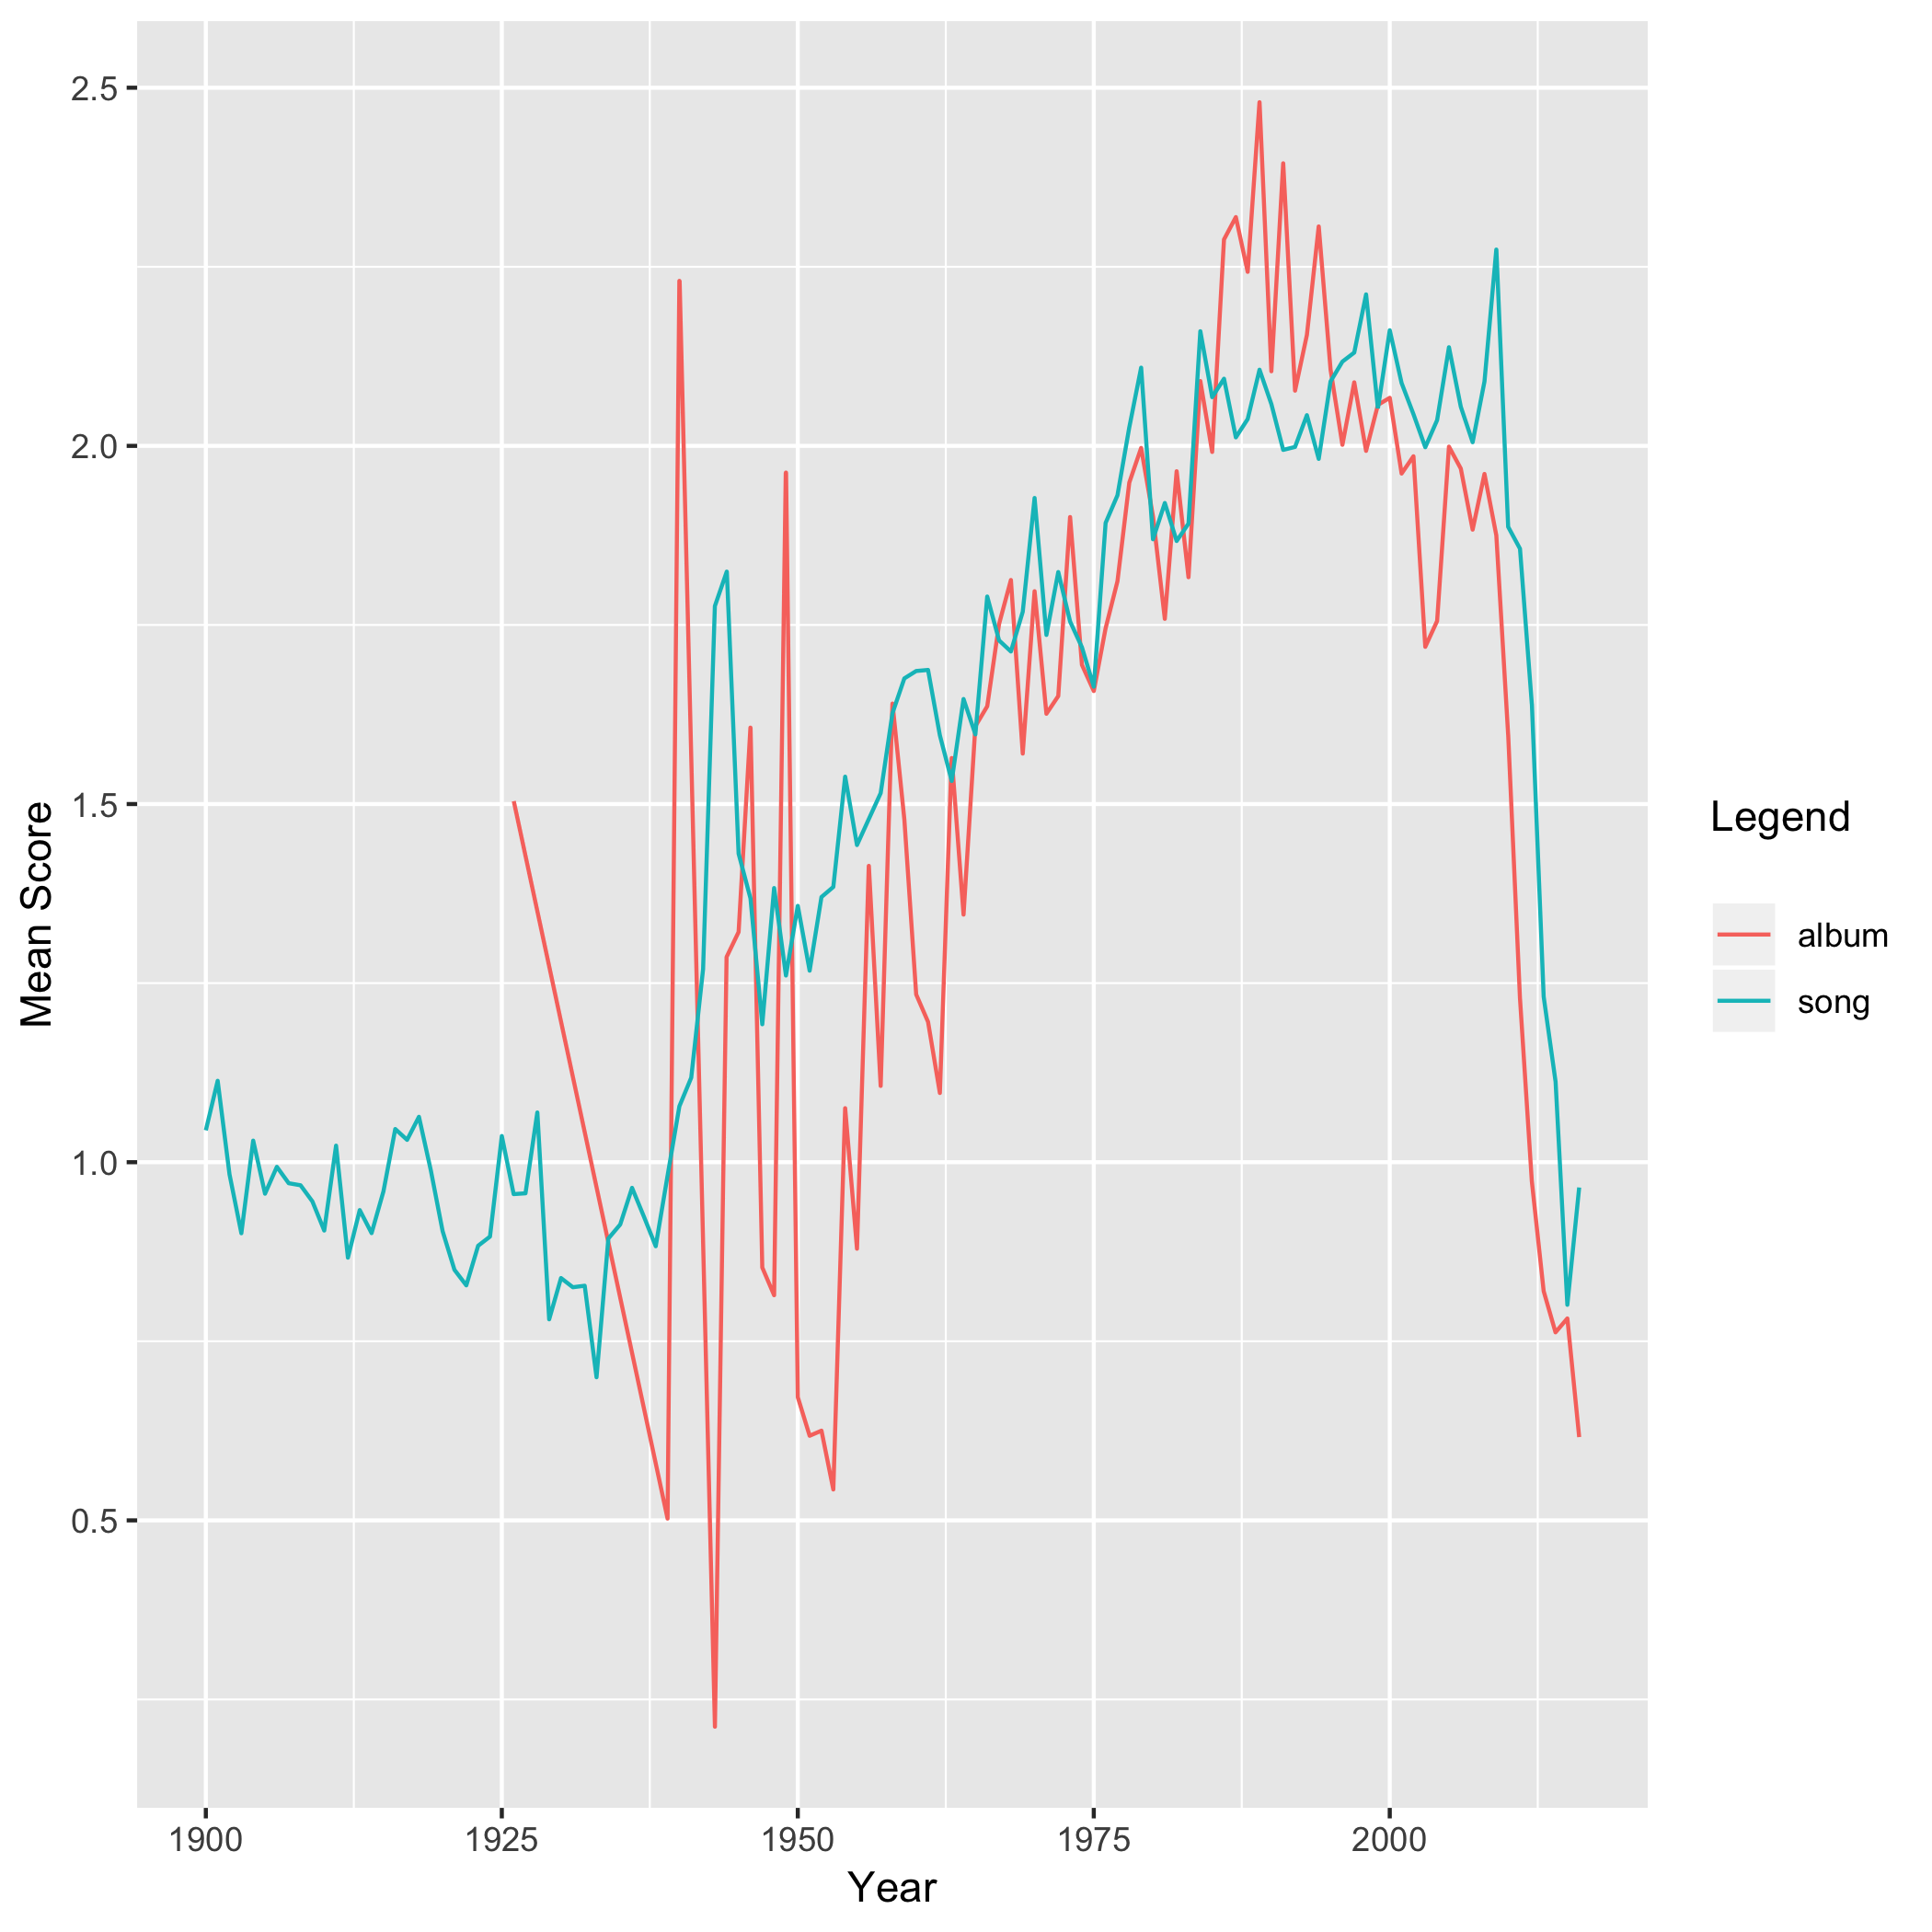
\includegraphics[width=0.5\textwidth]{songAlbumRates}
          \label{fig:q6}
        \end{SCfigure}

        Figure \ref{fig:q6} shows us that on the whole albums are rated lower than songs on a year-by-year basis, however one could argue that there is no real trend as especially around the late 60s/early 70s there was a large amount of variation in both.

\section{Critical Analysis}
Overall this was an interesting dataset to work with.
Finding trends across years is something that fascinates me about music, and this dataset enabled that superbly.
However, there could have been more.
A "genre" column could have lent a huge amount of scope for interesting visualisations.
As it was, there was somewhat limited scope for questions.
In terms of the development process, there was some time taken getting used to the dataset and working out what questions might be interesting to answer; the graph in Figure \ref{fig:q4p1} started out as a question by itself until it turned into the full question, and that was largely the story of the development process.
I would like to come back to this dataset again, however I would also like it to be perhaps somewhat more comprehensive.

\end{document}
